\newcommand{\Draft}{}
\newcommand{\Slide}{}
\newcommand{\PrintLecture}{1}
\newcommand{\PrintSolution}{1}
\newcommand{\MyCourse}{データサイエンスコース}
\newcommand{\MySemester}{春}
\newcommand{\MySubject}{ビジネス アナリティクス}
\newcommand{\MyClass}{第17回ー分類}% フォルダ名自動挿入

%
% 科目共通定義
%

\newcommand{\OpenIntro}
{\MyRef{OpenIntro Statistics}{https://www.openintro.org/book/os}}

\newcommand{\R}{\textbf{R}}
\newcommand{\RStudio}{\textbf{RStudio}}
\newcommand{\Excel}{\textbf{Excel}}
\newcommand{\cs}[1]{\textcolor{blue}{\texttt{#1}}} % Console prompt >

\newcommand{\ra}{\rightarrow}
\newcommand{\Ra}{\Rightarrow}

% Expectation E[X]
\def\E#1{E\big[#1\big]}
\def\S{\sum_{i=1}^n}

\newcommand{\B}{\hat{\beta}}
\newcommand{\SUM}{\sum_{i=1}^n}  % Summention from i=1 to n
\newcommand{\NH}{$\mathit{H}_0$} % Null hypthesis
\newcommand{\AH}{$\mathit{H}_1$} % Alternative hypothesis
\newcommand{\T}{\texorpdfstring{$t$}{}}% Student's t
\newcommand{\overtext}[3][1.5]{
  \mathrel{\overset{#2}{\scalebox{#1}[1]{$#3$}}}
}
\newcommand{\iid}{\overtext[2]{iid}{\sim}}
\newcommand{\convdist}{\overtext[2]{d}{\rightarrow}}
\newcommand{\convprob}{\overtext[2]{p}{\rightarrow}}
\newcommand{\as}[2]{\quad \text{as}\quad #1 \rightarrow #2}

\input{../../tex/hss_lualatex.tex}
\input{../../tex/hss_hyperref.tex}
\input{../../tex/hss_beamer.tex}

\setbeameroption{hide notes}
%\setbeameroption{show notes}
%\setbeameroption{show only notes}
%\setbeameroption{show notes on second screen=right}

\begin{document}

\maketitle

\MyFrame{}{\tableofcontents}

\section{時系列データ}

\MyFrame{}
{
  \MyDefinition{時系列データ}
  { 
    ある現象の時間的な変化を観測して得られた値の数列を\MyFill{時系列}といい,
    観測時間と観測値を共に記録したデータを\MyFill{時系列データ}という.
  }
 % \begin{minipage}{width=0.45\textwidth}
    \MyFig{0.5}{electricity_data.png}
 % \end{minipage}
 % \begin{minipage}{width=0.45\textwidth}
 %   \MyFig{0.7}{electricity_graph.png}
 % \end{minipage}
}

\MyFrame{}
{
  \MyDefinition{時系列グラフ}
  { 
    時系列データを用い,横軸に時間,
    縦軸にその時の値をとったグラフを\MyFill{時系列グラフ}という.
    \MyFill{折れ線グラフ}ともいう.
  }
  \MyFig{0.8}{electricity_graph.png}
}
\MyFrame{時系列グラフ}
{
  \MyAlert{注意点}
  {
    データ点とデータ点を結ぶ線は,観測していない時間の観測値の
    近似値としての意味合いを持つので,近似が不適切な場合は線で結ばないこと.
    その場合は,棒グラフが適している.
  }
}

\MyFrame{\insertsection}
{
  %\MyFig{1.1}{時系列データにおける変動の種類}
  %\MyRef
  %{【統計WEB】時系列データにおける周期変動}
  %{https://bellcurve.jp/statistics/course/23739.html}
  \MyDefinition{時系列データに含まれる変動の種類}
  {
   【傾向変動】中長期的傾向\\
   【周期変動】一日,一週間,季節間などで,周期的に繰り返される変動\\
   【不規則変動】上記以外のランダムな変動
  }
  傾向変動のことを\MyFill{トレンド}(trend variation)という.
  季節ごとの周期変動を\MyFill{季節変動}(seasonal variation)という.\\
  (参考)\\
  景気の変動のように周期は一定でないが上下の
  繰り返す変動を\MyFill{循環変動}(サイクル)という.
}

\MyFrame{時系列データに含まれる変動の種類}
{
  \MyFig{0.9}{variation_timeseries.png}
}

\MyFrame{周期変動(一日)}
{
  \MyFig{0.7}{variation_intraday.png}
}

\MyFrame{周期変動(一週間)}
{
  \MyFig{0.7}{variation_intraweek.png}
}

\section{時系列グラフ R演習}

\MyFrame{\insertsection}
{
  RStudio Cloudで,
  次のURLにあるソースコードを\red{タイプ}し時系列グラフを作成せよ.
  \alert{コピペすると記憶に定着しないためNG}
  \url{https://rpubs.com/tkdhss111/timeseries}
}

\MyFrame{}
{
  \MyFig{0.8}{timeseries_data.png}

}

\MyFrame{}
{
  \MyFig{0.8}{timeseries_src.png}

}

\MyFrame{}
{
  \MyFig{1.0}{timeseries_graph.png}

}

\section{時系列グラフ R課題}

\MyFrame{時系列グラフ R課題}
{
  電力使用量のデータを使いRで時系列グラフを作成せよ.
  \MyFig{0.7}{timeseries_hw_data.png}
}

\MyFrame{時系列グラフ R課題}
{
  \MyFig{1.0}{timeseries_hw_data2.png}
}

\MyFrame{\insertsection}
{
  図が完成したら,
  RStudioの右上のアイコン
  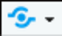
\includegraphics[width=8mm]{icon_publish.pdf}をクリックして,
  RPubsの入力画面で次の内容を入力し,
  www公開(publish)せよ.\\
  \alert{www公開されるので個人名など機微な情報は入力しないこと.}
  \begin{description}
    \item[Username] tiu学籍番号 (例)tiu22110001\\
    \item[Title] 時系列グラフ\\
    \item[Description] (空白/説明を入れてもよい)\\
    \item[Slug] timeseries
  \end{description}
  (職場で自分のソースコードとしてすぐに活用できるように,
    自分なりの補足説明やコメントを入れておきましょう.)\\
    ここでの方法に追加して,
    他のRのパッケージを使って作図したら評点に加えます.
}

\section{棒グラフ}

\MyFrame{\insertsection}
{
  \MyDefinition{棒グラフ}
  { 
    複数の項目を持つ数値データを用い,横軸に項目,縦軸に値をとり,
    値の大きさを四角い棒の高さで表現したグラフを
    \MyFill{棒グラフ}(barplot)という.
    縦横が逆の場合もある.
  }
  \MyFig{0.7}{barplot.png}
  \MyRef
  {【なるほど統計学園】棒グラフ}
  {https://www.stat.go.jp/naruhodo/4_graph/shokyu/bou-graph.html}
}

\MyFrame{\insertsection}
{
  \MyDefinition{積上棒グラフ}
  { 
    棒グラフで,1本の棒に,複数のデータを積み上げたものを
    \MyFill{積上棒グラフ}(stacked barplot)という.
  }
  \MyFig{0.7}{barplot_stacked.png}
  \MyRef
  {【なるほど統計学園】棒グラフ}
  {https://www.stat.go.jp/naruhodo/4_graph/shokyu/bou-graph.html}
}

\section{棒グラフ R演習}

\MyFrame{\insertsection}
{
  RStudio Cloudで,
  次のURLにあるソースコードを\red{タイプ}し棒グラフを作成せよ.
  \alert{コピペすると記憶に定着しないためNG}
  \url{https://rpubs.com/tkdhss111/barplot}
}

\MyFrame{}
{
  \MyFig{1.0}{barplot_data.png}

}

\MyFrame{R カラーパレット}
{
  \MyFig{0.8}{R_color_palette.png}
  \MyFig{0.7}{RGB.png}
  \MyRef{【ウィキペディア】RGB}{https://ja.wikipedia.org/wiki/RGB}
}

\MyFrame{}
{
  \MyFig{0.7}{fig/barplot_graph.png}
}

\MyFrame{}
{
  \MyFig{0.7}{fig/barplot_graph_stacked.png}
}

\MyFrame{}
{
  \MyFig{0.7}{fig/barplot_graph_grouped.png}
}

\end{document}
